%
% main.tex -- Paper zum Thema <punktgruppen>
%
% (c) 2020 Hochschule Rapperswil
%
\newcommand{\flippedA}{\raisebox{\fontcharht\font`a}{\scalebox{-1}[-1]{a}}}

\chapter[Crystal Math]{Crystal M\flippedA{}th\label{chapter:punktgruppen}}
\lhead{Crystal M\flippedA{}th}
\begin{refsection}
\chapterauthor{Naoki Pross, Tim T\"onz}

\section{Einleitung}

Es gibt viele Möglichkeiten sich in Kristallen zu verlieren.
Auch wenn man nur die mathematischen Betrachtungsweisen berücksichtigt, hat man noch viel zu viele Optionen sich mit Kristallen zu beschäftigen.
In diesem Kapitel wird daher der Fokus ``nur'' auf die Symmetrie gelegt.
Zu Beginn werden wir zeigen, was eine Symmetrie ausmacht und dass sie noch weit mehr in sich verbirgt als nur schön auszusehen.
Die vorgestellten Symmetrien sind äusserst gut geeignet, um die Grundeigenschaften eines Kristalles zu beschreiben.
Mit etwas kniffligen geometrischen Überlegungen kann man zeigen, was in der Welt der Kristallographie alles möglich ist oder nicht.
Diese erlauben alle möglichen Kristalle nach ihren Symmetrien in erstaunlich wenige Klassen zu kategorisieren.
Kategorien sind nicht nur für einen besseren Überblick nützlich, sondern kann man aus ihnen auch auf physikalische Eigenschaften schliessen.
Als spannendes Beispiel: Die Piezoelektrizität.
Piezoelektrizität beschreibt einen Effekt, ohne welchen diverse Altagsgegenständen nicht besonders nützlich wären.
Wie zum Beispiel sorgt er in den allermeisten Feuerzeugen für die Zündung.
Hiermit ist hoffentlich ein Funken Interesse geweckt um sich mit dem scheinbar trivialen Thema der Symmetrie auseinander zu setzten.

%% vim:linebreak breakindent showbreak=.. spell spelllang=de:

\section{Symmetrie}
Das Wort Symmetrie ist sehr alt und hat sich seltsamerweise von seinem
ursprünglichen griechischen Wort \(\mathrm{\Sigma\upsilon\mu\mu\varepsilon\tau\rho\iota\alpha}\)\footnote{\emph{Symmetr\'ia}: ein gemeinsames Mass habend, gleichmässig,verhältnismässig} fast nicht verändert.
In der Alltagssprache mag es ein locker definierter Begriff sein, in der Mathematik hat Symmetrie jedoch eine sehr präzise Bedeutung.
\begin{definition}[Symmetrie]
  Ein mathematisches Objekt wird als symmetrisch bezeichnet, wenn es unter einer bestimmten Operation invariant ist.
\end{definition}
Die intuitivsten Beispiele kommen aus der Geometrie, daher werden wir mit einigen geometrischen Beispielen beginnen.
Wie wir jedoch später sehen werden, ist das Konzept der Symmetrie eigentlich viel allgemeiner.

\begin{figure}
  \centering
  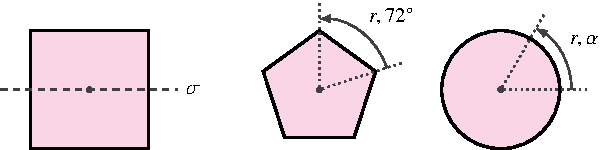
\includegraphics{papers/punktgruppen/figures/symmetric-shapes}
  \caption{
    Beispiele für geometrisch symmetrische Formen.
    \label{fig:punktgruppen:geometry-example}
  }
\end{figure}

\subsection{Geometrische Symmetrien}

In Abbildung \ref{fig:punktgruppen:geometry-example} haben wir einige Formen, die offensichtlich symmetrisch sind.
Zum Beispiel hat das Quadrat eine Gerade, an deren es gespiegelt werden kann, ohne sein Aussehen zu verändern.
Regelmässige Polygone mit \(n\) Seiten sind auch gute Beispiele, um eine diskrete Rotationssymmetrie zu veranschaulichen, was bedeutet, dass eine Drehung um einen Punkt um einen bestimmten Winkel \(360^\circ/n\) die Figur unverändert lässt.
Das letzte Beispiel auf der rechten Seite ist eine unendliche Rotationssymmetrie. Sie wird so genannt, weil es unendlich viele Werte für den Drehwinkel \(\alpha \in \mathbb{R}\) gibt, die die Form unverändert lassen.
Ein Objekt kann mehr als nur eine Symmetrie aufweisen.
Als Beispiel, kann das Quadrat in Abbildung \ref{fig:punktgruppen:geometry-example} nicht nur um \(\sigma\) sondern auch diagonal gespiegelt werden oder um \(90^\circ\) gedreht werden.
Fasst man die möglichen Symmetrien zusammen, entsteht eine Symmetriegruppe.

\begin{definition}[Symmetriegruppe]
  Seien \(g\) und \(h\) umkehrbare Operationen, sogenannte Symmetrieoperationen, die ein mathematisches Objekt unverändert lassen.
  Die Komposition \(h\circ g\) definieren wir als die Anwendung der Operationen nacheinander.
  Alle möglichen Symmetrieoperationen bilden unter Komposition eine Gruppe, die Symmetriegruppe genannt wird.
\end{definition}

Eine Gruppe benötigt ausserdem auch zwingend ein neutrales Element, welches wir mit \(\mathds{1}\) bezeichnen.
Die Anwendung der neutralen Operation ist gleichbedeutend damit, alles unverändert zu lassen.
Weiterhin muss in einer Gruppe für jede Operation \(g\) auch eine inverse Operation \(g^{-1}\) vorkommen, die intuitiv rückgängig macht, was \(g\) getan hat. % intuitiv weglassen oder anstelle sinnbildlich 
Somit ist \(\mathds{1}\) auch äquivalent dazu, eine Operation und dann ihre Inverse anzuwenden.
 Die Definition der Symmetriegruppe ist mit der Kompositionsoperation gegeben, sie wird aber auch oft als Multiplikation geschrieben.
Das liegt daran, dass in manchen Fällen die Zusammensetzung algebraisch durch eine Multiplikation berechnet wird.
Die Verwendung einer multiplikativen Schreibweise ermöglicht es, einige Ausdrücke kompakter zu schreiben, z.B.
durch Verwendung von Potenzen \(r^n = r\circ r \circ \cdots r\circ r\) für eine wiederholte Komposition.

\begin{definition}[Zyklische Untergruppe, Erzeuger]
  Sei \(g\) ein Element einer Symmetriegruppe \(G\).
  Alle möglichen Kompositionen von \(g\) und \(g^{-1}\) bilden eine sogenannte zyklische Untergruppe von \(G\), wobei \(g\) Erzeuger der Untergruppe genannt wird.
  Die von \(g\) erzeugte Untergruppe \(\langle g \rangle = \left\{ g^k : k \in \mathbb{Z} \right\}\) wird mit spitzen Klammern bezeichnet.
\end{definition}
\begin{beispiel}
  Um die Syntax zu verstehen, betrachten wir eine durch \(a\) erzeugte Gruppe \(G = \langle a \rangle\).
  Das bedeutet, dass \(G\) die Elemente \(a, aa, aaa, \ldots\) sowie \(a^{-1}, a^{-1}a^{-1}, \ldots\) und ein neutrales Element \(\mathds{1} = aa^{-1}\) enthält.
\end{beispiel}
\begin{beispiel}
  Als anschaulicheres Beispiel, können wir eine zyklische Untergruppe des \(n\)-Gon formalisieren.
  Wir bezeichnen mit \(r\) eine Drehung im Gegenuhrzeigersinn von \(360^\circ/n\) um einen Punkt.
  Diese Definition reicht aus, um die gesamte Symmetriegruppe
  \[
    C_n = \langle r \rangle
      = \left\{\mathds{1}, r, r^2, \ldots, r^{n-1}\right\}
  \]
  der Drehungen eines \(n\)-Gons zu erzeugen.
  Das liegt daran, dass wir durch die mehrfache Verwendung von \(r\) jeden Winkel erzeugen k\"onnen, der die Rotationssymmetrie bewahrt.
  In ähnlicher Weise, aber weniger interessant  enthält die Reflexionssymmetriegruppe \(\langle\sigma\rangle\) nur \(\left\{\mathds{1}, \sigma\right\}\), weil \(\sigma^2 = \mathds{1}\).
\end{beispiel}

Wenn wir diese Idee nun erweitern, können wir mit einem Erzeugendensystem
komplexere Strukturen aufbauen.

%@Naoki Are you ok with my grammar fixes I'm not 101% shore how to use the word Erzeugendensystem? 
\begin{definition}[Erzeugendensystem]
  Jede disktrete Gruppe kann durch eines oder mehrere ihrer Elemente generiert werden.
  Wir lassen \(g_1, g_2, \ldots, g_n\) erzeugenden Elemente einer Symmetriegruppe sein.
  Da es mehrere Erzeuger gibt, müssen auch die sogenannten Definitionsgleichungen gegeben werden, die die Multiplikationstabelle vollständig definieren.
  Die Gleichungen sind ebenfalls in den Klammern angegeben.
  Die erzeugenden Elementen bauen zusammen mit den Definitionsgleichungen ein Erzeugendensystem.
\end{definition}
\begin{beispiel}
  Wir werden nun alle Symmetrien eines \(n\)-Gons beschreiben, was bedeutet, dass wir die Operationen \(r\) und \(\sigma\) kombinieren.
  Die Definitionsgleichungen sind \(r^n = \mathds{1}\), \(\sigma^2 = \mathds{1}\) und \((\sigma r)^2 = \mathds{1}\).
  Die ersten beiden sind ziemlich offensichtlich.
  Die letzte wird oft auch als Inversion bezeichnet, weil die Anwendung von \(\sigma r\) dasselbe ist wie das Ziehen einer Linie von einem Punkt, die durch den Ursprung geht, und das Verschieben des Punktes auf die andere Seite des Nullpunkts.
  Wenn man dies zweimal macht, geht man zurück zum Anfangspunkt.
  Daraus ergibt sich die so genannte Diedergruppe 
  \begin{align*}
    D_n &= \langle r, \sigma : r^n = \sigma^2 = (\sigma r)^2 = \mathds{1} \rangle \\
      &= \left\{
          \mathds{1}, r, \ldots, r^{n-1}, \sigma, \sigma r, \ldots, \sigma r^{n-1}
      \right\}.
  \end{align*}
\end{beispiel}

Die Symmetrieoperationen, die wir bis jetzt besprochen haben, haben immer mindestens einen Punkt gehabt, der wieder auf sich selbst abgebildet wird.
Im Fall der Rotation war es der Drehpunkt, bei der Spiegelung die Punkte der Spiegelachse.
Dies ist jedoch keine Voraussetzung für eine Symmetrie, da es Symmetrien gibt, die jeden Punkt zu einem anderen Punkt verschieben können.
 Diesen Spezialfall, bei dem immer mindestens ein Punkt unverändert bleibt, nennt man Punktsymmetrie.
\begin{definition}[Punktgruppe]
  Wenn es einen Punkt gibt, der von jeder Gruppenoperation unverändert gelassen wird, ist die Symmetriegruppe eine Punktgruppe.
\end{definition}

\subsection{Algebraische Symmetrien}
Wir haben nun unseren Operationen Symbole gegeben, mit denen es tatsächlich möglich ist, Gleichungen zu schreiben.
Die anschliessende Frage ist dann, ob wir bereits mathematische Objekte haben, mit denen wir Gleichungen schreiben, die sich auf die gleiche Weise verhalten.
Die Antwort lautet natürlich ja.
Um es formaler zu beschreiben, werden wir einige Begriffe einführen.
\begin{definition}[Gruppenhomomorphismus]
  \(G\) und \(H\) seien  Gruppen mit unterschiedlichen Operationen \(\diamond\) bzw.
  \(\star\).
  Ein Homomorphismus\footnote{ Für eine ausführlichere Diskussion siehe \S\ref{buch:grundlagen:subsection:gruppen} im Buch.} ist eine Funktion \(f: G \to H\), so dass für jedes \(a, b \in G\) gilt \(f(a\diamond b) = f(a) \star f(b)\).
  Man sagt, dass der Homomorphismus \(f\) \(G\) in \(H\) transformiert.
\end{definition}
\begin{beispiel}
  Die Rotationssymmetrie des Kreises \(C_\infty\), mit einem unendlichen Kontinuum von Werten \(\alpha \in \mathbb{R}\), entspricht perfekt dem komplexen Einheitskreis.
  Der Homomorphismus \(\phi: C_\infty \to \mathbb{C}\) ist durch die Eulersche Formel \(\phi(r) = e^{i\alpha}\) gegeben.
\end{beispiel}

\begin{definition}[Darstellung einer Gruppe]
  Die Darstellung einer Gruppe ist ein Homomorphismus, der eine Symmetriegruppe auf eine Menge von Matrizen abbildet.
  \[
    \Phi: G \to \operatorname{GL}_n(\mathbb{R}).
  \]
  Äquivalent kann man sagen, dass ein Element aus der Symmetriegruppe auf einen Vektorraum \(V\) wirkt, indem man definiert \(\Phi : G \times V \to V\).
\end{definition}
\begin{beispiel}
  Die Elemente \(r^k \in C_n\), wobei \(0 < k < n\), stellen abstrakt eine Drehung von \(2\pi k/n\) um den Ursprung dar.
  Die mit der Matrix 
  \[
    \Phi(r^k) = \begin{pmatrix}
      \cos(2\pi k/n) & -\sin(2\pi k/n) \\
      \sin(2\pi k/n) &  \cos(2\pi k/n)
    \end{pmatrix}
  \]
  definierte Funktion von \(C_n\) nach \(O(2)\) ist eine Darstellung von \(C_n\).
  In diesem Fall ist die erste Gruppenoperation die Komposition und die zweite die Matrixmultiplikation.
  Man kann überprüfen, dass \(\Phi(r^2 \circ r) = \Phi(r^2)\Phi(r)\).
\end{beispiel}

\section{Kristalle}
%einleitung sollte noch an das ende von der Symmetrie angepasst werden
Unter dem Begriff Kristall sollte sich jeder ein Bild machen können.
Wir werden uns aber nicht auf sein Äusseres fokussieren, sondern was ihn im Inneren ausmacht.
Die Innereien eines Kristalles sind glücklicherweise relativ einfach definiert.
\begin{definition}[Kristall]
    Ein Kristall besteht aus Atomen, welche sich in einem Muster arrangieren, welches sich in drei Dimensionen periodisch wiederholt.
\end{definition}

\begin{figure}
    \centering
    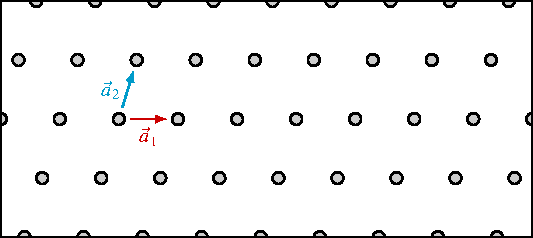
\includegraphics[]{papers/punktgruppen/figures/lattice}
    \caption{
        Zweidimensionales Kristallgitter.
        \label{fig:punktgruppen:lattice}
    }
\end{figure}
\subsection{Kristallgitter}
Ein zweidimensionales Beispiel eines solchen Muster ist Abbildung \ref{fig:punktgruppen:lattice}.
Für die Überschaubarkeit haben wir ein simples Motiv eines einzelnen grauen Punktes dargestellt und betrachten dies nur in zwei Dimensionen.
Die eingezeichneten Vektoren \(\vec{a}_1\) und \(\vec{a}_2\) sind die kleinstmöglichen Schritte im Raum bis sich das Kristallgitter wiederholt.
Wird ein beliebiger grauer Gitterpunkt in \ref{fig:punktgruppen:lattice} gewählt und um eine ganzzahlige Linearkombination von \(\vec{a}_1\) und \(\vec{a}_2\) verschoben, endet er zwangsweise auf einem Gitterpunkt, wenn nicht wieder am selben Ort.
Im dreidimensionalen Raum können alle Gitterpunkte mit derselben Idee und einem zusätzlichen Vektor \(\vec{c}\) also
\[
	\vec{r} = n_1 \vec{a}_1 + n_2 \vec{a}_2 + n_3 \vec{a}_3 = \sum_i n_i \vec{a}_i
\]
erreicht werden sofern \(n_1,n_2,n_3 \in \mathbb{Z}\) sind.
Sind die Vektoren  \(\vec{a}_1\), \(\vec{a}_2\), \(\vec{a}_3\) gegeben, ist ein Kristallgitter eindeutig beschrieben, weswegen sie auch als Grundvektoren bekannt sind.

\subsection{Translationssymmetrie} 
Da sich das ganze Kristallgitter wiederholt, wiederholen sich auch dessen Eigenschaften periodisch mit den Grundvektoren.
Sollte man sich auf einem Gitterpunkt in einem Kristall aufhalten, ist es unmöglich zu wissen, auf welchem Gitterpunkt man sich befindet, da die Umgebungen aller Punkte identisch sind. 
Mit anderen Worten: Jedes Kristallgitter $ G $ ist \emph{Translationssymmetrisch} in der Translation 
\[
    \vec{Q}_i(G) = G + \vec{a}_i
\] wobei der Vektor $\vec{a}_i$ ein Grundvektor sein muss.
Da die Translationssymmetrie beliebig oft mit allen Grundvektoren angewendet werden kann, 
können wir auch sagen, dass alle Verschiebungen um eine Linearkombination 
der Vektoren $\vec{a}_1$ , $\vec{a}_2$ und $\vec{a}_3$ erlaubt sind oder kurz, um $\vec{r}$. 
Verschiebungen um $\vec{r}$ bewirken demnach keine Veränderungen, 
solange wir ein unendlich grosses Kristallgitter verschieben.

\subsection{Limitierte Kristallsymmetrien} \label{txt:punktgruppen:Translationssymmetrie}
 Die Translationssymmetrie ist wohl keine grosse Überraschung, wenn man die Abbildung \ref{fig:punktgruppen:lattice} betrachtet.
 Was nicht direkt ersichtlich ist, dass bei beliebigen Grundvektoren nicht beliebige Symmetrien erstellt werden können.
 Die geforderte Translationssymmetrie eines Kristalles schränkt weitere Symmetrien deutlich ein.
  
\begin{figure}
    \centering
    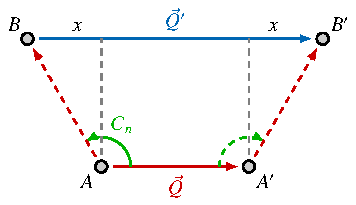
\includegraphics[]{papers/punktgruppen/figures/combine-symmetries}
    \caption{
        Translations und Rotationssymmetrisches Kristallgitter
    }
    \label{fig:punktgruppen:rot-geometry}
\end{figure}

\begin{satz}
   Die Rotationssymmetrien eines Kristalls sind auf 2-fach, 3-fach, 4-fach und 6-fach beschränkt.
   Mit anderen Worten: Es sind nur Drehwinkel von
    0\(^{\circ}\),
    60\(^{\circ}\),
    90\(^{\circ}\),
    120\(^{\circ}\) und
    180\(^{\circ}\)
   erlaubt.
\end{satz}

\begin{proof}
 In Abbildung \ref{fig:punktgruppen:rot-geometry} sehen wir Gitterpunkte und deren Zusammenhänge.

 \begin{itemize}
     \item  \(A\) ist unser erster Gitterpunkt. 

     \item  \(A'\) ist gegeben, weil wir \(A\) mit der Translation \(\vec{Q}\) um einen Grundvektor verschieben und wir wissen, 
            dass nach einer Translation wieder ein Gitterpunkt an der verschobenen Stelle sein muss.
     \item \(B\) entsteht, weil wir die Rotationssymmetrie \(C_n\) auf den Punkt \(A\) anwenden.
         Dadurch dreht sich das ganze Gitter um den Winkel \(360^\circ/n\). 
         Für uns bedeutet dies lediglich, dass unser zweiter Punkt \(A'\) abgedreht wird.
         An der neuen Position \(B\) von \(A'\) muss also auch ein Punkt des Gitters sein, um die Rotationssymmetrie zu erfüllen.
     \item \(B\) ist unser Name für diesen neuen Punkt.
         Da auch die Eigenschaften des Kristallgittes periodisch mit dem Gitter sein müssen, dürfen wir \(C_n\) auch auf \(A'\) anwenden.
         Also wenden wir \(C_n\) invertiert\footnote{Eine Rotationssymmetrie muss auch in die inverse Richtung funktionieren.
         Genauere Überlegungen hierzu werden dem Leser überlassen, da sich die Autoren nicht explizit mit dieser Frage Auseinander gesetzt haben.} 
         auch auf \(A'\) an. 
         Dies dreht \(A\) auf einen neuen Punkt.
     \item \(B'\) ist kein zufälliger Name für diesen neuen Punkt, denn wir wissen, dass zwischen allen Punkten eine Translationssymmetrie bestehen muss.
         Die  Translationssymmetrie zwischen \(B\) und \(B'\) ist hier als \(\vec{Q}'\) bezeichnet.
 \end{itemize}  
 Mit den gegebenen Punkten lassen sich geometrische Folgerungen ziehen.
 Wir beginnen, indem wir die Länge der Verschiebung \(|\vec{Q}| = Q\) setzen und \(|\vec{Q}'| = Q'\).
 Aus Abbildung \ref{fig:punktgruppen:rot-geometry} ist ersichtlich, dass \(Q' = Q + 2x\).
 Da \(\vec{Q}\) eine Translation um ein Grundvektor ist , muss \(\vec{Q}'\) ein ganzes vielfaches von \(\vec{Q}\) sein.
 Demnach auch die Längen
 \[
    Q' = nQ = Q + 2x
 \]
 Die Strecke \(x\) lässt sich auch mit hilfe der Trigonometrie und dem angenommenen Rotationswinkel \(\alpha\) ausdrücken:
 \[
    nQ = Q + 2Q\sin(\alpha - \pi/2)
 \]
 Wir können durch \(Q\) dividieren um unabhängig von der Läge des Grundvektors zu werden, was auch Sinn macht, 
 da eine Skalierung eines Kristalles seine Symmetrieeigenschaften nicht tangiert.
 Zusätzlich können wir den Sinusterm vereinfachen.
 \[
     n = 1 - 2\cos\alpha \quad\iff\quad
     \alpha = \cos^{-1}\left(\frac{1-n}{2}\right)
 \]
 Dies schränkt die möglichen Rotationssymmetrien auf 
 \(
     \alpha \in \left\{ 0^\circ, 60^\circ, 90^\circ, 120^\circ, 180^\circ\right\}
 \)
ein.
\end{proof}

\begin{figure}
    \centering
    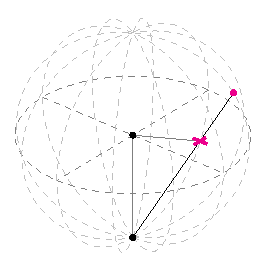
\includegraphics[height=6cm]{papers/punktgruppen/figures/stereographic-projections}
    \caption{
      Stereografische Projektion einer \(C_{i}\) Symmetrie. Es wird eine Linie vom magentafarbenen Punkt auf der oberen Hälfte der Kugel zum Südpol gezogen.
      Wo die Linie die Ebene schneidet (\(z = 0\)), ist die Projektion des Punktes.
      Die Koordinaten der Projektionen sind einfach zu berechnen: ein Punkt auf eine Kugel mit Radius \(r\) mit den Koordinaten \(x, y, z,\) wird auf \(xr/(r + z), yr/(r + z)\) projiziert.
      Für den orangefarbenen Punkt unterhalb des Äquators wird die Linie zum Nordpol gezogen und die Projektionsformel hat stattdessen einen Nenner von \(r - z\).
    }
    \label{fig:punktgruppen:stereographic-projections}
\end{figure}

\subsection{Kristallklassen}

Vorgehend wurde gezeigt, dass in einem zweidimensionalen Kristallgitter nicht alle Symmetrien möglich sind.
 Mit weiteren ähnlichen Überlegungen kann gezeigt werden, dass Kristalle im dreidimensionalen Raum nur auf genau 32 Arten rein punktsymmetrische Symmetriegruppen bilden können.
 Diese 32 möglichen Symmetriegruppen scheinen durchaus relevant zu sein, denn sie werden unter anderem als Kristallklassen bezeichnet.
 Die 32 möglichen Kristallklassen sind auf Abbildung \ref{fig:punktgruppen:Kristallkassen} zu sehen.
 Die Darstellung von dreidimensionalen Punktsymmetrien wurde mit der stereographischen Projektion ermöglicht (siehe Abbildung \ref{fig:punktgruppen:stereographic-projections}), wobei die gestrichelten Klassen aus Gründen der Überschaubarkeit nicht im Detail gezeichnet wurden.


\begin{figure}
    \centering
    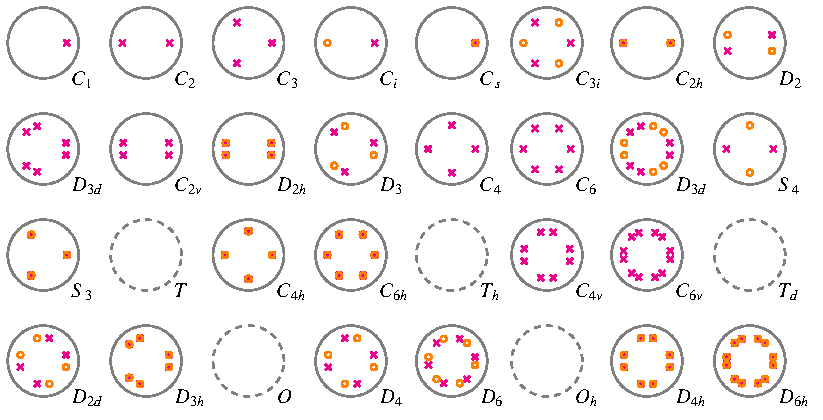
\includegraphics[]{papers/punktgruppen/figures/projections}
    \caption{Kristallklassen mit zugehörigem Schönflies-Symbol}
    \label{fig:punktgruppen:Kristallkassen}
\end{figure}

\subsubsection{Schönflies-Symbilok}

Jede der 32 Kristallklassen auf der Abbildung \ref{fig:punktgruppen:Kristallkassen} ist mit ihrem zugehörigen Schöönflies-Symbol bezeichnet.
 Die Schönflies-Symbolik stammt von dem Mathematiker Arthur Moritz Schönflies, welcher sich unter anderem mit der Klasifizierung der Punktgruppen auseinandergesetzt hat.
 Er hat Untergruppen gebildet, welche als Grossbuchstaben in Abbildung \ref{fig:punktgruppen:Kristallkassen} zu sehen sind.
 Da nicht alle Symmetriegruppen in Kristallen möglich sind, werden nicht alle Untergruppen von Schönflies verwendet.
 Es ist nur die Drehgruppe \(C\), Diedergruppe \(D\), Drehspiegelgruppe \(S\), Tetraedergruppe \(T\) und die Oktaedergruppe \(O\).
 Für die eindeutige zuweisung in eine Kristallklasse werden noch identifizierende Merkmale als Subskript notiert.
 Bei der Untergruppe \(C\) werden beispielsweise die möglichen Rotationssymmetrien gezeigt.
 Dank Abschintt \ref{txt:punktgruppen:Translationssymmetrie} wissen wir, wieso auf \(C\) nur ganz bestimmte Subskripte folgen, Weol das Subskript \(n\) von \(C_n\) zeigt, dass es sich um eine \(n\)-fache Rotationssymmetrie handelt.
 Daher darf \(C_5\) auf der Abbildung \ref{fig:punktgruppen:Kristallkassen} nicht vorkommen darf, da \(360^\circ/5 =  72^\circ\) was nach Abschnitt \ref{txt:punktgruppen:Translationssymmetrie} in einem Kristall keine mögliche Rotationssymmetrie ist.
 Sind im Subskript Buchstaben, definieren diese weitere Symmetrieeigenschaften der Klasse.
 Wie zum Beispiel ein Inversionszentrum\footnote{Ein Objekt mit Inversionszentrum ist Punktsymmetrisch im Inversionszentrum.} \(i\) oder eine horizontale\footnote{Als Orientierungspunkt wird die Symmetrieachse höchster Ordnung (\(n\)) als vertikal definiert} Spiegelachse \(h\).
 Zu beachten ist jedoch, dass manche Symmetriegruppen mit mehreren Schönflies-Symbolen beschieben werden können.
 \(C_{3i}\) beschreibt genau das selbe wie \(S_6\), da eine dreifache Rotationssymmetrie mit einem Inversionszentrum einer sechsfachen Drehspiegelsymmetrie entspricht.




%% vim:spell spelllang=de showbreak=.. breakindent linebreak:

\section{Piezoelektrizität}
\rhead{Piezoelektrizität}
\index{Piezoelektrizität}%
Die Piezoelektrizität ist die spannende Eigenschaft, dass gewisse Kristalle eine elektrische Spannung erzeugen, wenn mechanischer Druck auf sie ausgeübt wird.
\index{elektrische Spannung}%
\index{mechanischer Druck}%

\begin{figure}
    \centering
    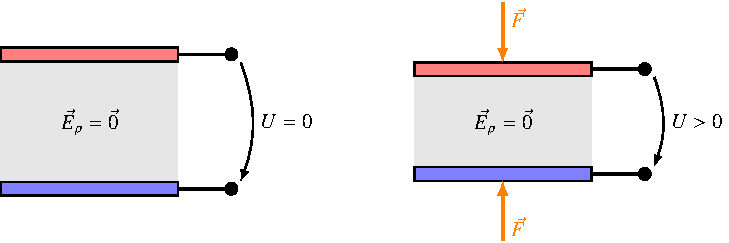
\includegraphics[]{papers/punktgruppen/figures/piezo} %das Efeld mit Naoki disskutieren, müssen sicher gehen, dass es mit jenen in Abbildung Piezo aufbau übereinstimmt
    \caption{Piezoelektrisches Material in Ruhe und unter Druck}
    \label{fig:punktgruppen:basicPiezo}
\end{figure}

\subsection{Polarisierung}
\index{Polarisierung}%
Piezoelektrizität basiert darauf, dass zwischen den Oberflächen des Kristalles ein Ladungsungleichgewicht entsteht (siehe Abbildung\ref{fig:punktgruppen:basicPiezo}).
Dieses Ungleichgewicht resultiert, weil durch den mechanischen Druck auf der einen Oberfläche des Kristalles positive Ionen näher an die Oberfläche gelangen, wärend auf der gegenüberliegenden Seite dasselbe mit negativen Ionen passiert.
\index{Ionen}%
Es besitzt jedoch nicht jeder Kristall eine atomare Struktur, welche sich unter Druck genau so verformt.
Der Aufbau und somit auch die Symmetrie des Kristalles sind daher relevant für die Entstehung dieses Effektes.


\begin{figure}
    \centering
    \begin{tabular}{c |c}
      \subfigure[][\label{fig:punktgruppen:atoms-piezo}]{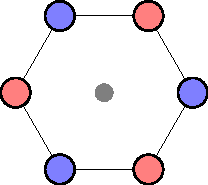
\includegraphics{papers/punktgruppen/figures/atoms-piezo-still}} &
      \subfigure[][\label{fig:punktgruppen:atoms-grid}]{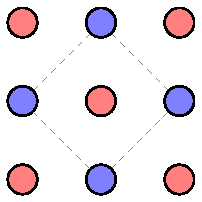
\includegraphics{papers/punktgruppen/figures/atoms-grid-still}} \\
      \subfigure[][\label{fig:punktgruppen:atoms-piezo-fv}]{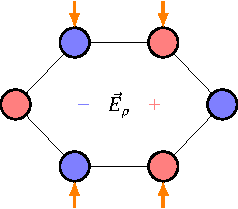
\includegraphics{papers/punktgruppen/figures/atoms-piezo-force-vertical}}
      \hspace{2mm}
      \subfigure[][\label{fig:punktgruppen:atoms-piezo-fh}]{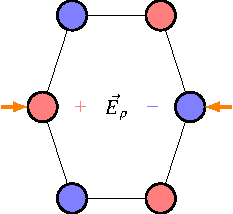
\includegraphics{papers/punktgruppen/figures/atoms-piezo-force-horizontal}}
      \hspace{3mm} & \hspace{3mm}
      \subfigure[][\label{fig:punktgruppen:atoms-grid-f}]{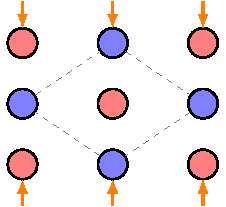
\includegraphics{papers/punktgruppen/figures/atoms-grid-force}} \\
    \end{tabular}
    \caption{
        Kristallstrukturen mit und ohne piezoelektrischer Eigenschaft.
    }
    \label{fig:punktgruppen:atomPiezo}
\end{figure}

\subsection{Atomarer Aufbau}

Die Polarisation entsteht an der Oberfläche eines Kristalles, die Erklärung dazu finden wir jedoch im atomaren Aufbau.
Wir wollen dazu die verschiedenen Kristallstrukturen auf Abbildung \ref{fig:punktgruppen:atomPiezo} diskutieren.
In Abbildung \ref{fig:punktgruppen:atomPiezo} gilt für alle Strukturen, dass rote Kreise positive Ionen und blaue negative Ionen repräsentieren.
Struktur \subref{fig:punktgruppen:atoms-piezo} zeigt ein piezoelektrisches Material in Ruhe.
Struktur \subref{fig:punktgruppen:atoms-piezo-fv} ist dasselbe Kristallgitter, jedoch wird es senkrecht belastet.
Eingezeichnet ist auch das elektrische Feld, welches entsteht, weil die Ladungsträger ganz links und rechts weiter auseinander gedrückt werden.
\index{elektrisches Feld}%
\index{Ladungsträger}%
Als Hilfe zur Vorstellung kann man \subref{fig:punktgruppen:atoms-piezo-fv} zwischen zwei leitende Platten setzen, so wird ersichtlich, dass mit wachsendem Druck eine negative Ladung an die rechte Platte gedrückt wird, während sich die positiven Ionen weiter entfernen.
 

Die Struktur \subref{fig:punktgruppen:atoms-grid} ist nicht piezoelektrisch.
Dies wird ersichtlich, wenn man \subref{fig:punktgruppen:atoms-grid} unter Druck setzt und sich die Struktur zu \subref{fig:punktgruppen:atoms-grid-f} verformt.
Setzt man \subref{fig:punktgruppen:atoms-grid-f} gedanklich auch zwischen zwei leitende Platten, scheint es, als würden rechts mehr positive Ionen in die Platte gedrückt werden und links umgekehrt.
Dies ist aber nicht mehr der Fall, wenn sich die Struktur nach oben und unten periodisch wiederholt.


Struktur \subref{fig:punktgruppen:atoms-piezo-fh} zeigt \subref{fig:punktgruppen:atoms-piezo} in unter horizontaler Belastung.
Was zwischen \subref{fig:punktgruppen:atoms-piezo-fv} und \subref{fig:punktgruppen:atoms-piezo-fh} zu beobachten ist, dass die entstandene Ladungsdifferenz orthogonal zu der angelegten Kraft entsteht, im Gegensatz zu \subref{fig:punktgruppen:atoms-piezo-fh}.
Daraus kann man schliessen, dass \subref{fig:punktgruppen:atoms-piezo} keine Rotationssymmetrie von \(90^\circ\) besitzen kann, weil die Eigenschaften der Struktur sich bei einer \(90^\circ\) Drehung ändern.
Das Fehlen dieser Rotationssymmetrie bestätigt sich auch wenn \subref{fig:punktgruppen:atoms-piezo} als Hexagon betrachtet wird.
 

\subsection{Punktsymmetrie}

Piezoelektrische Kristalle können nicht punktsymmetrisch sein.
Kristallgitter, bei welchen eine Punktspiegelung eine symmetrische Operation ist, können keine piezoelektrische Kristalle bilden.
In Abbildung \ref{fig:punktgruppen:atomPiezo} ist bewusst \subref{fig:punktgruppen:atoms-piezo} ein nicht punktsymmetrischer Kristall mit einem punktsymmetrischen \subref{fig:punktgruppen:atoms-grid} verglichen worden.
Als vereinfachte Erklärung kann man sich wieder das Bild eines Kristalles wie \subref{fig:punktgruppen:atoms-piezo} vor Augen führen, welcher unter Druck auf der einen Seite negative und der anderen Seite positive Ionen an seine Oberfläche verdrängt.
Spiegelt man nun den Kristall um den Gitterpunkt in der Mitte des Kristalles, so würden die negativen Ionen auf den positiven auf der anderen Seite landen, was der Definition einer Symmetrie deutlich widerspricht.


\subsection{Vom Kristall zum Feuer}

Piezoelektrizität hat durchaus Nutzen im Alltag.
Feuerzeuge welche nicht auf dem Prinzip beruhen einen Zündstein abzuschleifen, sondern ohne Verschleiss auf Knopfdruck einen Zündfunken erzeugen, basieren auf dem Prinzip der Piezoelektrizität.
\index{Feuerzeug}%
Drückt der Nutzende auf den Zündknopf, spannt sich eine Feder bis zu einer konfigurierten Spannung.
Drückt der Nutzende stärker zu, entspannt sich die Feder schlagartig und beschleunigt mit der gespeicherten Energie ein Hammer, welcher auf das Piezoelement aufschlägt.
Der augenblicklich hohe Druck sorgt an den Piezokontakten für eine eben so kurze aber hohe elektrische Spannung.
Die Spannung reicht aus, um eine Funkenstrecke zu überwinden und so eine entflammbares Gas zu entzünden.

Sollte der Leser eines Tages in die Situation geraten, in welcher er zwei verschiedene Kristalle vor sich hat und ein piezoelektrisches Feuerzeug bauen musst, wobei bekannt ist, dass der eine eine Punktsymmetrie aufweist, empfiehlt es sich, sich mit dem anderen zu versuchen.



\nocite{punktgruppen:pinter-algebra}
\nocite{punktgruppen:sands-crystal}
\nocite{punktgruppen:lang-elt2}
\nocite{punktgruppen:ouchem}
\nocite{punktgruppen:restriction}

\printbibliography[heading=subbibliography]
\end{refsection}
